\documentclass[11pt]{article}
\usepackage{acl2014}
\usepackage{times}
\usepackage{url}
\usepackage{latexsym}
\usepackage[utf8]{inputenc} %http://depling.org/depling2015/formats/depling2015latex/depling2015latex.zip
\usepackage{color}
\usepackage{xspace}
\usepackage{url}

\usepackage{amsmath}
%%\usepackage{color}
\usepackage{amsfonts}
\usepackage{amssymb}
\usepackage{graphicx}
\usepackage{multirow}


\def \xxx#1{\textbf{\textcolor{red}{xxx: #1}}}
\def \todo#1{\textbf{\textcolor{red}{todo: #1}}}
\def\equo#1{``#1''}

\def\Tref#1{Table~\ref{#1}}
\def\Fref#1{Figure~\ref{#1}}
\def\Sref#1{Section~\ref{#1}}
\newcommand{\out}[1]{\textcolor[rgb]{0.8,0.8,0.8}{\textbf{#1}}}
\newcommand{\ml}[1]{\textcolor{red}{\raisebox{.2ex}{\tiny ML:~}#1}}
\def\footurl#1{\footnote{\url{#1}}}

%\usepackage[left=2cm,right=2cm,top=2cm,bottom=2cm]{geometry}

\title{Targeted Paraphrasing for Machine Translation Evaluation}

\author{Petra Barančíková \\
  Institute of Formal and Applied Linguistics \\
  Charles University in Prague, Faculty of Mathematics and Physics\\
  Malostranské náměstí 25, Prague, Czech Republic \\
  {\tt barancikova@ufal.mff.cuni.cz} \\}

\date{}
%
%This paper describes Parmesan, our submission to the 2014 Workshop on Statistical Machine Translation (WMT) metrics task for evaluation English-to-Czech translation. 
%We show that the Czech Meteor Paraphrase tables are so noisy that they actually can harm the performance of the metric. However, they can be very useful after extensive filtering in targeted paraphrasing of Czech reference sentences prior to the evaluation.
%Parmesan first performs targeted paraphrasing of reference sentences, then it computes the Meteor score using only the exact match on these new reference sentences. It shows significantly higher correlation with human judgment than Meteor on the WMT12 and WMT13 data. However, this result was not confirmed by this year's data.

\begin{document}

\maketitle
\begin{abstract}
This thesis is focused on improving an accuracy of machine translation to 
Czech language using targeted paraphrasing. We develop and compare several 
approaches for creating new synthetic references that are closer in wording to 
a~corresponding machine translations. 

These new reference sentences make evaluation using traditional metrics 
more reliable as they lack of paraphrase and free word order support.

After implementation, the system for generating new synthetic references will 
be beneficial not only for MT evaluation, but mainly inside MT systems for 
improved tuning and development of the systems. This way, it will directly 
influence the quality of machine translation itself.

%Trade-off between simplicity and quality of MT metric!!
\end{abstract}

\section{Introduction}
The need for quality automatic machine translation (MT) evaluation is as old as
the machine translation itself. It is essential for objective evaluation during
development of a MT system as well as comparison of different MT systems.

The traditional human evaluation while being the most reliable has serious 
drawbacks. Not only it is time-consuming and expensive, but more importantly
it is highly dependent on the person annotating and the inter-annotator 
agreement is generally low  \cite{wmt13}. Moreover, it is practically 
impossible to repeat the evaluation with the same results \cite{bojar-kniha}.
%, although there were recently successful attempts to overcome this problem 
%using crowdsourcing techniques. [\markcite{{\it Callison-Burch}, 2009]} and 
%[\markcite{{\it Bentivogli et al.}, 2011]} demonstrate that the average score of 
%high number of non-expert low-paid annotators shows high agreement with gold 
%standards provided by expert annotators in various natural language processing 
%(NLP) tasks including machine translation evaluation.

Due to being slow and unreproducible, it is impossible to use human evaluation
for tuning and development of MT systems. Well-performing automatic MT 
evaluation metrics are essential precisely for these tasks. The pioneer metrics 
correlating well with human judgment were BLEU \cite{bleu} and NIST \cite{nist}. 
They are computed based on n-gram overlap between the MT output (hypothesis) and 
one or more corresponding reference sentences, i.e., translations made by a human 
translator.

Despite its age, BLEU still remains de facto standard metric for MT evaluation 
and tuning because of its simplicity and language independence, even though 
other, better-performing metrics exist (\newcite{wmt13-metrics}, 
\newcite{wmt14}). \todo{pridat novejsi clanky} \newcite{callison2006re} shows that 
correlation of BLUE with human judgment is not as high as previously thought.
% This is particular valid at a sentence level (Blatz et al. 2003).
%Post:  BLEU’s relative language indepen- dence, its ease of computation, and its reason- able correlation with human judgments have led to its adoption as the dominant metric for ma- chine translation research. 
%Post: This is of course not to claim there are no problems with BLEU. Its weaknesses abound, and much has been written about them (cf.  \cite{callison2006re}; \cite{reiter-2018-structured}). 

Furthermore, obtaining reference sentences is labour intensive and 
expensive,\footnote{For example, production of reference translation  at~the 
Linguistic Data Consortium is complicated process involving translation 
by~professional agencies based on elaborate guidelines and detailed quality 
control \cite{strassel}.} thus the standard practice is using only one 
reference sentence and BLEU then tends to perform badly. 

As there are many translations of a single sentence, even a perfectly correct 
hypothesis might get a low score due different wording and disregarding 
synonymous expressions (see \Fref{example_of_BLEU_malfunction}). This is 
especially valid for morphologically rich languages with free word order 
like the Czech language. \cite{bojar-tackling-sparse-data}

%Russo-Lassner
%While human evaluation of machine translation (MT) output remains the most reliable method to assess translation quality, it is a costly and time consuming process. The development of automatic MT evaluation metrics enables the rapid assessment of system output. By providing immediate feedback on the effectiveness of various techniques, these metrics have guided machine translation research and have facilitated rapid advances in the state of the art. In addition, automatic evaluation metrics are useful in comparing the performance of multiple MT systems on a given translation task, as demonstrated by the DARPA TIDES research program. Since automatic evaluation metrics are meant to serve as a surrogate for human judgments, their quality is determined by how well they correlate with assessors’ preferences and how accurately they predicts human judgments.
%Although current methods for automatically evaluating MT output do not require humans to assess individual system output, humans are nevertheless needed to generate a number of “reference translations”. The quality of machine-generated translations is determined by automatically comparing system output against these references. Despite numerous variations, which we will discuss in the next section, all current automatic evaluation metrics are based on the simple idea of matching substrings (i.e., n-grams) from machine output with substrings from the reference translations. This substring matching approach has obvious drawbacks: it does not account for combinations of lexical and syntactic differences that might occur between a perfectly fluent and accurately-translated machine output and a human reference translation (beyond variations already captured by the different reference translations themselves). Moreover, the set of human reference translations is unlikely to be an exhaustive inventory of “good translations” for any given foreign language sentence. Therefore, it would be highly desirable to have an MT evaluation metric capable of automatically determining equivalences in meaning without relying on exact substring matches.
%We propose a novel approach to automatic machine translation evaluation based on paraphrase identification. The quality of machine-generated output can be viewed as the extent to which the conveyed meaning matches the semantics of the reference translations, independent of substrings they may share. In short, all paraphrases of human-generated references should be considered “good” translations. We have implemented this idea in a statistical model of human preferences that combines features from existing automatic evaluation metrics with features that have proven to be useful in the paraphrase identification task. Results show that exploiting paraphrase identification techniques results in a statistically significant improvement in correlation with human judgments at the sentence level, measured against baselines that use only existing automatic metrics.

\begin{figure*}[tb]
\begin{center}
\begin{tabular}{ll}
 Original sentence &  \begin{tabular}{l}
  	\textit{Banks are testing payment by mobile telephone} \\
	\end{tabular}  \\
 \hline
 
 MT output & \begin{tabular}{llllll}
 			\textit{Banky} & \textit{zkou\v sej\'i} & \textit{platbu} & \textit{pomoc\'i} & \textit{mobiln\'iho} & \textit{telefonu} \\
 			Banks & are testing & payment & with help & mobile & phone \\
			\end{tabular} \\
 & \begin{tabular}{l}
  	Banks are testing payment by mobile phone \\
	\end{tabular} \\

 \hline
 Reference sentence & \begin{tabular}{llll}
 			\textit{Banky} & \textit{testuj\'i} & \textit{placen\'i} & \textit{mobilem} \\
 			Banks & are testing & paying & by mobile phone \\
			\end{tabular} \\
 &  \begin{tabular}{l}
  	Banks are testing paying by mobile phone \\
	\end{tabular}
 
\end{tabular}
\caption{Example from WMT12 - Even though the translation is grammatically 
correct and the meaning of both sentences is very similar, it doesn't contribute 
to the BLEU score. There is only one unigram overlapping.}
\end{center}
\label{example_of_BLEU_malfunction}
\end{figure*}

As the main task of an MT metric is essentially to decide whether a reference
sentence is a paraphrase of a given hypothesis, our goal is to achieve higher 
accuracy of MT evaluation by targeted paraphrasing of reference sentences., 
i.e. creating a new synthetic reference sentence that is still correct and 
keeps the meaning of the original sentence but at the same time it is closer in 
wording to the MT output. BLEU and other string-based metrics performs more 
reliable using these new references. %(TODO: nejak preformulovat)

The structure of the thesis is as follows: in the next section, we present 
other work in paraphrasing for MT evaluation. In \Sref{Data}, we introduced
the data we use for our experiments. In sections \ref{lrec} and \ref{MT}, 
we show paraphrasing based on phrase substitutions and machine translation 
itself. Finally, we conclude with avenues for further work.

\section{Related Work}
----

https://github.com/awslabs/sockeye/ tree/master/contrib/sacrebleu
pip3 install sacrebleu

The situation is even worsened by the fact, that the BLEU score is reported inconsistenly. \cite{post-2018-call} point out that the 

 Although people refer to “the” BLEU score, BLEU is in fact a param- eterized metric whose values can vary wildly with changes to these parameters. These pa- rameters are often not reported or are hard to find, and consequently, BLEU scores be- tween papers cannot be directly compared. I quantify this variation, finding differences as high as 1.8 between commonly used configu- rations. The main culprit is different tokeniza- tion and normalization schemes applied to the reference. Pointing to the success of the pars- ing community, I suggest machine translation researchers settle upon the BLEU scheme used by the annual Conference on Machine Trans- lation (WMT), which does not allow for user- supplied reference processing, and provide a new tool, SACREBLEU,1 to facilitate this.
 
 Bleu is ot a single metric, it requires a number of parameters, these include the number of references used (and the computation of the length penalty if more references used), the maximum n-gram length, smoothing applied to 0-counts n-grams. But basically most of these are moot - most often there is only one reference, maximum n-gram length is virtually always four and since BLEU is corpus level, it is rare that there are any zero counts - i.e. more theoretical problem.
 
 
 It's largely affected by preprocessing (normalization, tokenizatin,...). BLEU scores are often reported as being tokenized or detokenized. But for comput- ing BLEU, both the system output and reference are always tokenized; what this distinction refers to is whether the reference preprocessing is user- supplied or metric-internal (i.e., handled by the code implementing the metric), respectively. And since BLEU scores can only be compared when the reference processing is the same, user-supplied preprocessing is error-prone and inadequate for comparing across papers.
 
 Difference up to 1.5 BLEU points based on different preprocessing.
 
 
 Scores computed against differenty-processed references are not comparable. Papers vary in the hidden parameters and schemes they use, yet often do not report them.
 
 He introduces a Python package SacreBLEU, which automatically downloads and stores references for common test sets and thus introducing a "protective layer" between them and the user. It also provides a number of other featueres such as reporting a version string which records the parameters used and which can be included in published papers

----
\cite{reiter-2018-structured} shows:
- for MT is text-level correlation poor, but reasonably well for system level
- that correlation of BLEU with ranking based on human assesment differs very much during many years of WMT(07 to 16) evaluation (e.g. EN-DE Spearman: 0.26 (07), 0.58 (08), -0.43(09), 0.39(10), ..), it is very much depnedent on the detauks if the details of the evaluation (corpora, human ranking assesment).
- BLEU was originally proposed for diagnostic evaluation of MT systems, that is, as a technique for allowing researchers and developers to quckly "weed out bad ideas from good ideas" (\cite{bleu}, page 311). I thing the surveyed papers support this use of BLE, since most of the system-level BLEU-human correlationns for MT reported Medium or High.
- there is a wide range of correlation of BLEU and human judgment even in very similar tasks, this suggests the correlation is dependent on contextual factors
- BLEU has technological biases that we do not understand. This is especially worrying as new technologies such as neural networks becme more prominent, we do not know if BLEU is "fair" to such technologies. 

https://pdfs.semanticscholar.org/301c/621fba608afa5c04ac149eb16c6a6e621289.pdf

\cite{callison2006re} 


\cite{wmt16} n Figure 3–5, we plotted the human evaluation result against everybody’s favorite metric BLEU. Although these two metrics correlate generally well, the plots clearly suggest that a fair comparison of systems of different kinds cannot rely on automatic scores. Rule-based systems receive a much lower BLEU score than statistical systems (see for instance English–German, e.g., PROMT-RULE). The same is true to a lesser degree for statistical syntax-based systems (see English– German, UEDIN-SYNTAX vs. UEDIN-PBMT).

https://pdfs.semanticscholar.org/7d45/d353baf9c3b49963886c37af8d735a624ec1.pdf?_ga=2.167828257.1279602481.1565166754-1247173902.1546618752


https://arxiv.org/pdf/1905.12752.pdf
\cite{roy2019}

https://www.aclweb.org/anthology/N16-3013
\cite{napoles-etal-2016-sentential}
https://cwiki.apache.org/confluence/pages/viewpage.action?pageId=65142863 - vyzkouset

https://arxiv.org/pdf/1901.03644.pdf
https://arxiv.org/pdf/1804.06059.pdf
https://www.aclweb.org/anthology/N16-3013

There are two attitudes towards solving the problem - one is to change the 
automatic metric itself to be tolerant to other sentence representation and the
other one is to pre-process automatically the reference sentence via 
paraphrasing.

\subsection{Automatic Metrics}
Second generation metrics Meteor \cite{meteor-wmt:2014}, TERp \cite{terp} and 
ParaEval \cite{paraeval2} still largely focus on a n-gram overlap while 
including other linguistically motivated resources. They utilize paraphrase 
support using their own paraphrase tables and show higher correlation with 
human judgment than BLEU.


Meteor is available for several languages including Czech. It explicitly 
addresses weaknesses of BLEU -- it takes into account recall, distinguishes 
between functional and content words, allows language-specific tuning of 
parameters and many others. Its  basic setting of Meteor for evaluation 
of~Czech sentences offers two levels of matches -- exact and paraphrase. As we 
show further (see \Sref{parmesan}), its paraphrase tables are so noisy that 
they actually harm the performance of the metric, as it can award mistranslated 
and even untranslated words.

String matching is hardly discriminative enough to reflect the human perception 
and there is growing number of metrics that compute their score based on rich 
linguistic features -- matching based on parse trees, POS tags or textual 
entailment (e.g. \newcite{liu:2005}, \newcite{owczarzak:2007}, 
\newcite{amigo:2009}, \newcite{Pado09}, \newcite{machacek:2011}). 

These metrics shows better correlation with human judgment, but their wide 
usage is limited by being complex and language-dependent. As a result, there is
a trade-off between linguistic-rich strategy for better performance and 
wide applicability of simple string level matching.

%the development of automatic MT evaluation metrics falls into  a  dilemma of choosing 
%the string level matching for wide application or selecting the linguistic-rich strategy
%for better performance.  Faced with an evaluation task involving multiple  languages as 
%in WMT campaigns [Callison-Burch   et al., 2008; 2009; 2010], a language independent
% metric of high performance is more desirable.

\subsection{Sentence paraphrasing}
% Mozna tu zminit, ze tech metod parafrazovani je hromada (viz Lin a Pantel)
% krome pri ev
Targeted paraphrasing for MT evaluation is introduced in~\newcite{kauchak}. 
They focus on lexical substitution in Chinese-to-English translations. They 
select all pairs of words for which one word appears in a reference sentence, 
second word in a hypothesis, but none of them in both. They keep only 
pairs of synonymous words, i.e. words appearing in the same WordNet 
\cite{wordnet} synset. Each such a pair of words was further contextually 
evaluated. For every confirmed synonym, a new reference sentence is created by 
placing it to the reference sentence on the position of its synonym.

This solution is not directly applicable to the Czech language. As Czech 
belongs to~inflective languages with rich morphology, a Czech word has 
typically many forms and the correct form depends heavily on its context, 
e.g., morphological cases of nouns depend on verb valency frames. Changing 
a~single word may result into not grammatical sentence. Therefore, we do not 
attempt to~change a~single word in~a~reference sentence but we focus 
on~creating one single correct reference sentence.

There is many other application for paraphrases in the MT field. Paraphrases 
are utilized for translating out-of-vocabulary words and increase quality of MT 
systems trained on sparse data \cite{Callison-Burch:2006}, \cite{Marton:2009} or 
enlarge training data \cite{nakov2008improved}.
\newcite{madnani2010circle} and \newcite{mehay2012shallow} show that single 
translation augmented by targeted paraphrases can successfully replace up to
four additional human reference translation in the tuning phase of a MT system.
 
%\xxx{Wubben} 

\section{Data}
\label{Data}
\subsection{Text Data}
We perform our experiments on data sets from the English-to-Czech translation 
task of WMT12 \cite{wmt12}, WMT13 \cite{wmt13}. The data sets contain 
13/14\footnote{We use only 12 of them because two of them 
(FDA.2878 and online-G) have no human judgments.} files with Czech outputs 
of different MT systems. Each file contains 3003/3000 sentences.

In addition, each data set contains one file with corresponding reference 
sentences and one with original English source sentences. We perform 
morphological analysis and tagging of the hypotheses and the reference 
sentences using Morče \cite{morce:2007}.

The human judgment of hypotheses is available as a relative ranking of 
performance of five systems for~a~sentence. We calculated the absolute 
performance of every system by the “$ > $ others” method \cite{bojar-grains}, 
which was the WMT12 official system score. It is computed as 
$ \frac{wins}{wins+loses} $, ties among several systems are ignored. We use 
this score as a human judgment in further evaluation.
%We refer to this interpretation of human judgment as 
%\textit{silver standard} to distinguish it from the official system scores, which were 
%computed differently each year (here referred to as \textit{gold standard}).

\subsection{Sources of Paraphrases}
\label{meteori}
We make use of two existing sources of Czech paraphrases -- the Czech WordNet 
1.9 PDT \cite{czech-wordnet} and the Meteor Paraphrase Tables \cite{meteor-tables}. 
%Czech PPDB \cite{ppdb} became available only recently and we plan to use it in 
%further research.

The \textbf{Czech WordNet 1.9 PDT} is derived from the WordNet \cite{wordnet} 
by automatic translation followed by manual verification. It~contains rather 
high quality lemmatized paraphrases. However, their amount is~insufficient for 
our purposes - it contains only 13k pairs of synonymous lemmas. % and 
%- only one paraphrase per four sentences on~average is found in~the data. % (see \Tref{number_of_substitutions}).  

On~the other hand, Czech \textbf{Meteor Paraphrase tables} are quite the 
opposite of Czech WordNet -- they are large in size, but contain a lot of 
noise, as they were constructed automatically via \textit{pivoting} 
\cite{pivoting}. The pivot method is an inexpensive way of acquiring paraphrases 
from large parallel corpora. It is based on the assumption that two phrases 
that share a meaning may have a same translation in a foreign language 
\cite{dyvik}.

The noise is particularly high among the multiword paraphrases -- for %TODO podle lopatkove the high for multiw...
example: \textit{svého názoru} (its opinion) and \textit{šermovat rukama a 
mlátit neviditelného} (to flail one's arms and to beat the invisible one) are 
selected as a paraphrase. We experimented with several methods of reducing
the noise in the multi-word paraphrases, however, none of them outperforms
omitting them completely \cite{barancikova:2014}.
 
Among one-word paraphrases the noise is sparser, but the paraphrase tables  %TODO podle lopatkove the high for multiw...
still contains pairs such as \textit{pijavice} (a leech) - \textit{1873}
or \textit{afgh\'{a}nci} (Afghans) - \textit{š\v{t}astně} (happily). 
However, the biggest problem is that most of synonymous pairs were just 
different word forms of the same lemma. 

We perform automatic filtering among the one-word paraphrases in the 
Meteor table in the following way. Using Morče, we first perform morphological  %TODO markete se nelibi: in the following way.
analysis of all one-word pairs and replace the word forms with their lemmas. We 
keep only pairs of different lemmas. Further, we dispose of pairs of words that 
differ in their parts of speech (POS)\footnote{With a single exception -- 
paraphrases consisting of numeral and corresponding digits, e.g., 
\textit{osmnáct} (eighteen) and \textit{18} - \textit{osmnáct} has the part of 
speech \textit{C}, which is designated for numerals, \textit{18} is marked with 
\textit{X} meaning it is an unknown word for the morphological analyzer.} or
~contain an unknown (typically foreign) word.

In this way we have reduced 684k paraphrases in~the original Czech Meteor 
Paraphrase tables to~only 32k pairs of lemmas. We refer to~this paraphrase
table as~to~\textit{filtered Meteor}.

\section{Simple substitution paraphrasing}
\label{lrec}
We experiment with several algorithms for paraphrasing reference sentences. 
The method in this section is widely based on \newcite{kauchak}. We start with 
a basic algorithm for phrase substitution from a hypothesis to a reference. 
We experiment with different phrase lengths and two methods for phrase 
selection.

The newly created reference may be non grammatical because of the direct
substitutions from the hypothesis, thus we employ Depfix \cite{depfix}, 
a~system for automatic correction of~grammatical errors that appear often 
in~English-to-Czech MT outputs. 

\subsection{Candidate Selection}
We select potential paraphrases using two different methods. The first one is a 
simple greedy search similar to~\newcite{kauchak}, the other one uses automatic 
word alignment for selecting corresponding segments of~the reference sentence 
and the hypothesis.

\subsubsection*{Simple Greedy Method}
Let $ w_1,...,w_m $, $ r_1,..., r_n $ be the hypothesis and the reference 
sentence, respectively. We performed their tagging and extracted sets of lemmas 
 $ W_{L} $, $ R_{L} $. Then, one-word paraphrase candidates are chosen as:
$$ C_{L} = \lbrace (r,w) | r \in R_{L} \smallsetminus W_{L} \wedge w \in W_{L}
\smallsetminus R_{L}  \rbrace $$

Multi-words candidates $ C_M $ are selected analogically from all sequences 
of words from the reference sentence and from the hypothesis. Maximum phrase 
length is seven words (as is the length of~the longest paraphrases in 
the data). % Formally:
%
%\begin{gather*}
%C_{M} = \lbrace (<r_i,..,r_{i+x}>, <w_j,...,w_{j+y}>) | \: 1 \leq i \leq n-x \: \wedge \\ 
% \: 1~\leq~j \leq m-y  \: \wedge \: 0 \leq x,y \leq 6 \: \wedge \: (x \neq 0 \vee y \neq 0) \rbrace 
%\end{gather*}

\subsubsection*{Word and Phrase Alignments}
One possible way to make the algorithm more reliable is to restrict the 
application of paraphrases to words/phrases which are aligned to each other. We 
compute word alignment between the reference translation and MT system outputs 
using GIZA++ \cite{gizapp}.

However, if we used only our test data to create the alignment (13 x 3003 + 12 
x 3000 = 75039 sentence pairs), the alignment quality would be insufficient. In 
order to make the training data for word alignment larger, we take advantage of 
the fact that all outputs are translations of the same data and also add all 
pairs of system outputs to our data, creating over 1,000,000 \equo{artificial} 
sentence pairs. For example, the parallel data for WMT12 then looks as follows:

\begin{center}
\begin{tabular}{ll}
Source & Target \\
\hline
system 1 & system 2 \\
system 1 & system 3 \\
... & ...\\
system 1 & system 13 \\
system 1 & reference \\
system 2 & system 1 \\
system 2 & system 3 \\
... & ... \\
system 13 & reference \\
\end{tabular}
\end{center}

We also experiment with adding much larger synthetic parallel data created by
machine translation (note that we need Czech-Czech data) but there was no 
impact on the quality of paraphrasing so we follow the outlined approach which 
requires no additional data or processing.

The set of~one-word candidates $C_L$ is then simply the set of all word pairs 
such that there exists an alignment link between them. The set $C_M$ is 
extracted using phrase extraction for phrase-based MT, the standard consistency 
criterion is~applied \cite{Och99improvedalignment}.

\subsection{Paraphrasing}
We reduce the $ C_{M} $ to pairs contained in the multi-word Meteor tables and
$ C_{L} $ to Czech WordNet and the filtered Meteor. If there is a lemma 
contained in several pairs in $ C_{L} $, we  give preference to those found 
in~WordNet or even better in the intersection of paraphrases from WordNet and 
filtered Meteor.

We evaluate three different paraphrasing methods which differ in the order of
substitution.

%\begin{description}
\subsubsection*{One-word only}
%\item[One-word only] 
We proceed word by word from the beginning of the reference 
sentence to~its end. If a~lemma of~a~word appears as~the first member of~a~pair 
in reduced $ C_{L} $, it is replaced by~the word from hypothesis that has its lemma
as the second element of~that pair, i.e., paraphrase from the hypothesis. Otherwise, 
we keep the original word from the reference sentence.
\subsubsection*{One-word first}
%\item[One-word first] 
We use \textit{One-word only} and then we apply longer paraphrases.
We move ahead from the longest paraphrases to the shortest. That is because 
Meteor contains often even components of~phrases and we could substitute, instead of~whole 
phrase, only part of~it. We do not attempt to replace any word that was already changed.
\subsubsection*{Multi-word first}
%\item[Multi-word first] 
We substitute the longest confirmed paraphrases from
$ C_{M} $ and move to the shorter ones. We replace again only sequences that have not
been substituted yet. After this, we paraphrase remaining unchanged words
with the \textit{One-word only} method.
%\end{description}

\begin{table*}[tb]
\begin{center}

\textbf{WMT12}\\
\begin{tabular}{l|cc|cc}
\hline
\multirow{2}{*}{Method} & \multicolumn{2}{c|}{Greedy selection} & \multicolumn{2}{c}{Word alignment} \\
& No Depfix & Full Depfix  & No Depfix & Full Depfix \\
\hline
One-word only     & 0.804 & \textbf{0.834} & 0.794 & 0.815 \\
One-word first    & 0.788 & 0.825 & 0.763 & 0.800  \\
Multi-word first  & 0.755 & 0.813 & 0.761 & 0.795  \\
\end{tabular}

\vspace{10pt}
Baseline~correlation: \textbf{0.751}
\vspace{10pt}

\textbf{WMT13}\\
\begin{tabular}{l|cc|cc}
\hline
\multirow{2}{*}{Method} & \multicolumn{2}{c|}{Greedy selection} & \multicolumn{2}{c}{Word alignment} \\
& No Depfix & Full Depfix  & No Depfix & Full Depfix \\
\hline
One-word only     & 0.865 & \textbf{0.891} & 0.860 & 0.881  \\
One-word first    & 0.854 & 0.884  & 0.836 & 0.874 \\
Multi-word first  & 0.841 & 0.875  & 0.840 & 0.871  \\
\end{tabular}

\vspace{10pt}
Baseline~correlation: \textbf{0.834}
\caption{Correlation of the human judgment and BLEU on new references created
by the simple substitution method.}
\label{lrec_results}
\end{center}
\end{table*}

\subsection{Depfix}
As we substitute a word form directly from a hypothesis, it may happen that a 
resulting new reference is not grammatically correct. We rectify these errors 
by applying Depfix \cite{depfix} -- an automatic post-editing system which is 
able to fix Czech sentences containing grammatical errors.

Depfix was originally designed for post-editing outputs of English-to-Czech 
phrase-based machine translation. It consists of a set of~linguistically-motivated 
rules and a statistical component that correct various kinds of errors, especially 
in grammar (e.g. morphological agreement), using a range of natural language 
processing tools to analyse of the input sentences.

We observe that the errors that appear in the outputs of our paraphrasing 
algorithm are often similar to some errors appearing in outputs of phrase-based
machine translation systems, e.g errors in morphological agreement are very 
common. This makes Depfix an appropriate tool for fixing the errors, since 
typical grammar correcting tools, such as a grammar-checker in a word processor, 
focus on errors that are typical for humans, not for machines. 

\subsection{Results}
\begin{figure}[t]

\begin{center}
\scalebox{0.90}{
\begin{tabular}{ll}
 Source &  \begin{tabular}{l}
  	\textit{The location alone is classic.} \\
	\end{tabular} \\
 \hline
 
 Hypothesis & \begin{tabular}{llll}
 			\textit{Samotné} & \textit{místo} & \textit{je} & \textit{klasické.} \\
 			Actual & place & is & classic \\
			\end{tabular} \\
 &  \begin{tabular}{l}
  	The place alone is classic. \\
	\end{tabular} \\

 \hline
 Reference & \begin{tabular}{llll}
 			\textit{Už} & \textit{poloha} & \textit{je} & \textit{klasická.} \\
 			Already & position & is & classic. \\
			\end{tabular} \\
 &  \begin{tabular}{l}
  	The position itself is classic. \\
	\end{tabular}  \\ 

 \hline
  New ref. & \begin{tabular}{llll}
 			\textit{Už} & \textit{místo} & \textit{je} & \textit{klasická.} \\
 			Already & place & is & classic \\
			\end{tabular} \\
 &  \begin{tabular}{l}
  	*The place itself is classic. \\
	\end{tabular} \\
 \hline 
  Depfixed ref. & \begin{tabular}{llll}
 			\textit{Už} & \textit{místo} & \textit{je} & \textit{klasické.} \\
 			Already & place & is & classic \\
			\end{tabular} \\
 &  \begin{tabular}{l}
  	The place itself is classic. \\
	\end{tabular} \\
 \hline  
 
\end{tabular}}
\caption{Example of the \textit{One-word only} method. The~hypothesis is grammatically 
correct and has very similar meaning as the reference sentence. The new reference is closer 
in wording to the hypothesis, but there is no agreement between the noun and adjective. 
Depfix resolves the error and the final reference is correct and much similar to~the hypothesis.}
\label{lrec_example}
\end{center}
\end{figure}

Results of our method are presented in \Tref{lrec_results} as the Pearson 
correlation between human judgment and BLEU computed on our new references. 
All evaluated approaches outperform the~baseline (i.e., using the original 
reference sentences), the simplest one \textit{One-word only} performs 
best (\Fref{lrec_example} shows an example of this method).

 
We use a freely available implementation\footurl{http://www.cnts.ua.ac.be/~vincent/scripts/rtest.py} of \cite{meng:1992} to determine whether the difference in correlation
coefficients is statistically significant. The test shows that BLEU performs
better with our reference sentences with 99\% certainty. 

Multi-word paraphrases are very noisy and while they do bring the system 
outputs closer to the reference (the average BLEU score is higher), they 
often propose non-equivalent translations or violate the correctness of the 
sentence, thus blurring the differences between systems.

When paraphrasing is restricted by word alignment, all methods perform worse. 
As Table \ref{lrec_replaced} shows, the number of applied paraphrases is much lower: 
while the proportion of correct paraphrases is higher, their amount is reduced 
too much and overall, our technique is harmed by this restriction. 

\begin{table}[tb]
\begin{center}
\scalebox{0.85}{
\begin{tabular}{l|cc|cc}
\multicolumn{5}{c}{\textbf{WMT12}}\\
\hline
\multirow{2}{*}{Method} & \multicolumn{2}{c|}{Greedy selection} & \multicolumn{2}{c}{Word alignment} \\
& Words & Phrases & Words & Phrases \\
\hline
One-word only     & 1.59 & --   & 0.86 &  --  \\
One-word first    & 1.59 & 0.23 & 0.86 & 0.22 \\
Multi-word first  & 1.38 & 0.31 & 0.81 & 0.27 \\
\end{tabular}}

\vspace{10pt}

\scalebox{0.85}{
\begin{tabular}{l|cc|cc}
\multicolumn{5}{c}{\textbf{WMT13}}\\
\hline
\multirow{2}{*}{Method} & \multicolumn{2}{c|}{Greedy selection} & \multicolumn{2}{c}{Word alignment} \\
& Words & Phrases & Words & Phrases \\
\hline
One-word only    & 1.33 &  --  & 0.76 & --   \\
One-word first   & 1.33 & 0.20 & 0.76 & 0.20 \\
Multi-word first & 1.04 & 0.68 & 0.74 & 0.24 \\
\end{tabular}}
\caption{Average number of replaced words/phrases per sentence.}
\label{lrec_replaced}
\end{center}
\end{table}

On the other hand, applying Depfix is always beneficial, with the positive 
effects ranging from 0.021 up to 0.058. This supports our assumption of the 
importance of grammatical correctness of the created references.

Results on the data from WMT13 and WMT12 are very similar -- paraphrasing 
helps to increase the accuracy of the evaluation, even though the differences 
on the WMT13 data are not as~big due to much higher baseline. This is also 
reflected in~the smaller amount of substitutions.

\subsection{Meteor without paraphrase support}
\label{parmesan}
Based on the positive impact of filtering Meteor Paraphrase Tables for targeted
lexical paraphrasing of reference sentences, we experiment with the filtering 
them yet again, but this time as~an~inner part of~the Meteor evaluation metric 
(i.e. for the paraphrase match).

\begin{table*}[tb]
\begin{center}

\scalebox{0.99}{
\begin{tabular}{r|c|l}
setting & size & description of the paraphrase table \\
\hline
\textbf{Standard} & 684k & The original Meteor Paraphrase Tables \\
\textbf{One-word} & 181k & \textbf{Basic} without multi-word pairs\\
\textbf{Same POS} & 122k & \textbf{One-word} + only same part-of-speech pairs\\
\textbf{Different Lemma} & 71k & \textbf{Same POS} + only forms of different lemma\\
\textbf{Exact match} & 0 & No paraphrase tables\\
\textbf{WordNet} & 202k & Paraphrase tables generated from Czech WordNet\\
\end{tabular}
}
\caption{Different paraphrase tables for Meteor and their size (number of paraphrase pairs).}
\label{meteory}
\end{center}
\end{table*}

The filtering of~the paraphrase tables is performed analogically. We experiment
with six different settings that are presented in~\Tref{meteory}. All of them
are created by reducing the original Meteor Paraphrase tables, except for the 
setting referred to~as~\textbf{WordNet}, which has its paraphrase table 
generated from one-word paraphrases in Czech WordNet to all their possible 
word forms appearing in~CzEng \cite{czeng}.
%
%Prior paraphrasing reference sentences and using Meteor with the \textbf{No 
%paraphr.} setting for computing scores constitutes Parmesan -- our submission
%to the WMT14 \cite{wmt14} for evaluation English-to-Czech translation. In the 
%tables with results, Parmesan scores are highlighted by the box and the best 
%scores are in bold. % \xxx{podle lopatkovy preformulovat}

\begin{table*}[tb]
\begin{center}
%\scalebox{0.95}{
\begin{tabular}{l|cccccc}
\multicolumn{7}{c}{\textbf{WMT12}}\\
\hline
references & Standard & One-word & Same POS &  Different Lemma & Exact match & WordNet \\
\hline
Original references & 0.833 & 0.836 & 0.840 & 0.863 & 0.861 & 0.863 \\
Before Depfix & 0.905 & 0.908 & 0.911 & 0.931 & 0.931 & 0.931 \\
New references & 0.927 & 0.930 & 0.931 & 0.950 & \textbf{0.951} & \textbf{0.951} \\
%\hline
\end{tabular}
%} 

\vspace{10pt}

%\scalebox{0.95}{
\begin{tabular}{l|cccccc}
\multicolumn{7}{c}{\textbf{WMT13}}\\
\hline
references & Standard & One-word & Same POS & Different Lemma & Exact match & WordNet \\
\hline
Original references & 0.817 & 0.820 & 0.823 & 0.850 & 0.848 & 0.850 \\
Before Depfix  & 0.865 & 0.867 & 0.869 & 0.895 & 0.895 & 0.894 \\
New references & 0.891 & 0.892 & 0.893 & \textbf{0.915} & \textbf{0.915} & \textbf{0.915} \\
%\hline
\end{tabular}
%}
\caption{Pearson's correlation of Meteor and the human judgment on original reference sentences and sentences created by the \textit{One-word only} method.}
\label{meteor_results}
\end{center}
\end{table*}

The results of our experiments are presented in \Tref{meteor_results}, they are 
very consistent for WMT12 and WMT13. We show that independently of~a~reference 
sentence used, reducing the Meteor paraphrase tables in evaluation is always 
beneficial. The Meteor metric with exact match only on paraphrased references 
significantly outperforms Meteor with paraphrase support on original 
references.

\textbf{Diff. Lemma} and \textbf{WordNet} settings give the best results on the 
original reference sentences. That is because they are basically a limited 
version of the paraphrase tables we use for creating our new references, which 
contain both all different lemmas of the same part of speech from the Meteor 
Paraphrase tables and all lemmas from Czech WordNet.

The main reason of the worse performance of the metric when employing the 
Meteor Paraphrase tables is the noise. The metric may award even parts of the 
hypothesis left untranslated, as the original Meteor Paraphrase tables contain 
some English words and their Czech translations as paraphrases. There are for
~example pairs: \textit{pšenice} - \textit{wheat}\footnote{In all examples the 
Czech word is the correct translation of the English side.}, \textit{vůdce} - 
\textit{leader}, \textit{vařit} -	\textit{cook}, \textit{poloostrov} - 
\textit{peninsula}.

\section{Paraphrasing using Machine Translation}
\label{MT}
While the one-word substitution method offers good results, it is very limited. 
We would like to be able to use longer paraphrases, word order changes, switch 
between active and passive construction, etc.

For this purpose, we employ machine translation itself -- there are many tools 
for MT and there is a close resemblance between translation and paraphrasing. 
They both attempt to preserve the meaning of a sentence, the first one between 
two languages and the second one within a single language by different word 
choice. It seems only natural to attempt to adjust some MT tools to translate 
within a single language for targeted paraphrasing. 

We describe this attempt on two types of MT systems -- phrase-based and 
rule-based. Initially, we experiment with the freely available SMT system 
Moses \cite{moses}. However, the results of this method are inconclusive. 
In the view of errors appearing in the new paraphrased sentences, we propose 
another solution -- targeted paraphrasing using a rule-based translation system 
included in the NLP framework Treex \cite{treex}.

\subsection{Paraphrasing via Moses}
Moses is a freely available statistical machine translation engine. 
In~a~nutshell, statistical machine translation involves the following phases: 
creating language and translation models, parameter tuning and decoding. 
We use Moses in the phrase-based setting. Simple scheme of Moses is presented
in \Fref{moses_simple}.

A language model is responsible for a correct word order and grammatical 
correctness of the translated sentence. A translation model (a phrase table) 
supplies all possible translations of a word or a phrase or in our case, all 
possible paraphrases. Models are assigned weights which are learned during the 
parameter tuning phase.

During the decoding phase, all these models are combined to maximize 
$ \sum_i \lambda_i \phi_i (\bar{f},\bar{e}) $, where  $ \lambda_i $ is a weight 
of the sub-model $ \phi_i $ and $ \bar{f},\bar{e} $ is a hypothesis and 
a source sentence, respectively. In our case, we want to make a reference 
sentence closer to a corresponding machine translation output -- $ \bar{e} $ is 
the reference sentence and $ \bar{f} $ is a new synthetic reference.

Moses with this setting could create paraphrases, but they would be just 
random paraphrases of the reference sentence -- their similarity to our 
original hypotheses would not be guaranteed. Therefore, we also add a new 
feature for targeted paraphrasing to Moses.


\begin{figure*}
\begin{center}

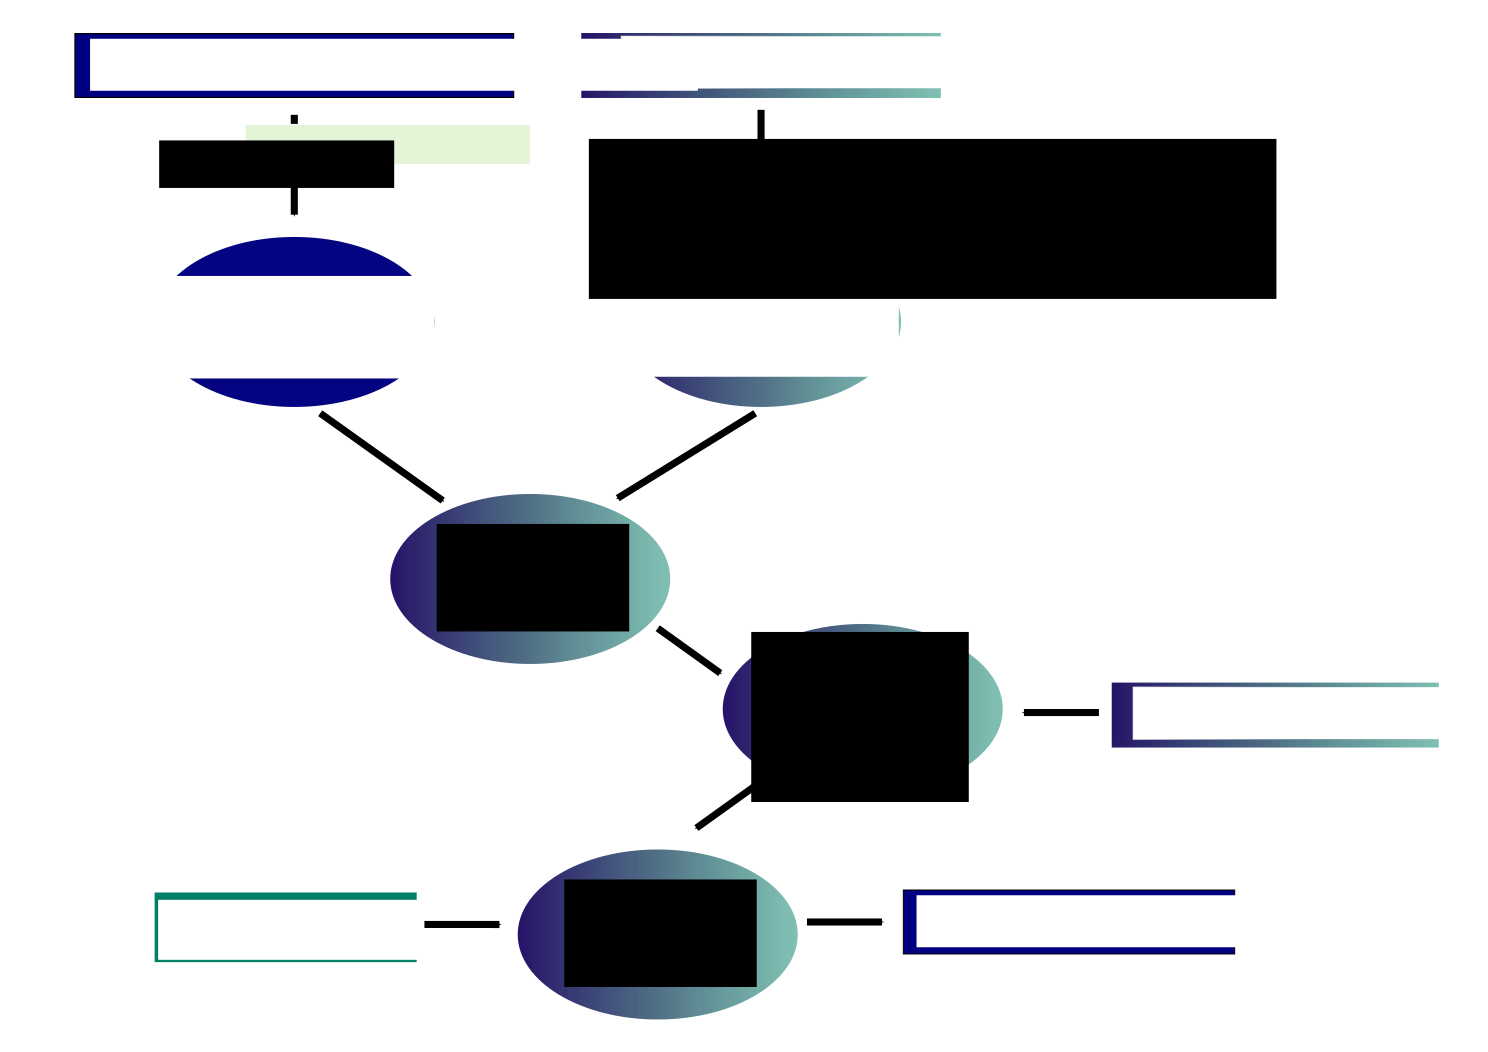
\includegraphics[scale=0.3]{moses.png} 
\caption{Simplified scheme of the translation system Moses. The blue colour 
represents a target language and the green colour represents a source language.}
\label{moses_simple}

\vspace{30pt}

\includegraphics[scale=0.65]{moses_translation_tables.png} 
\caption{Excerpt from the Enhanced Meteor table.}
\label{moses_tables}

\vspace{30pt}
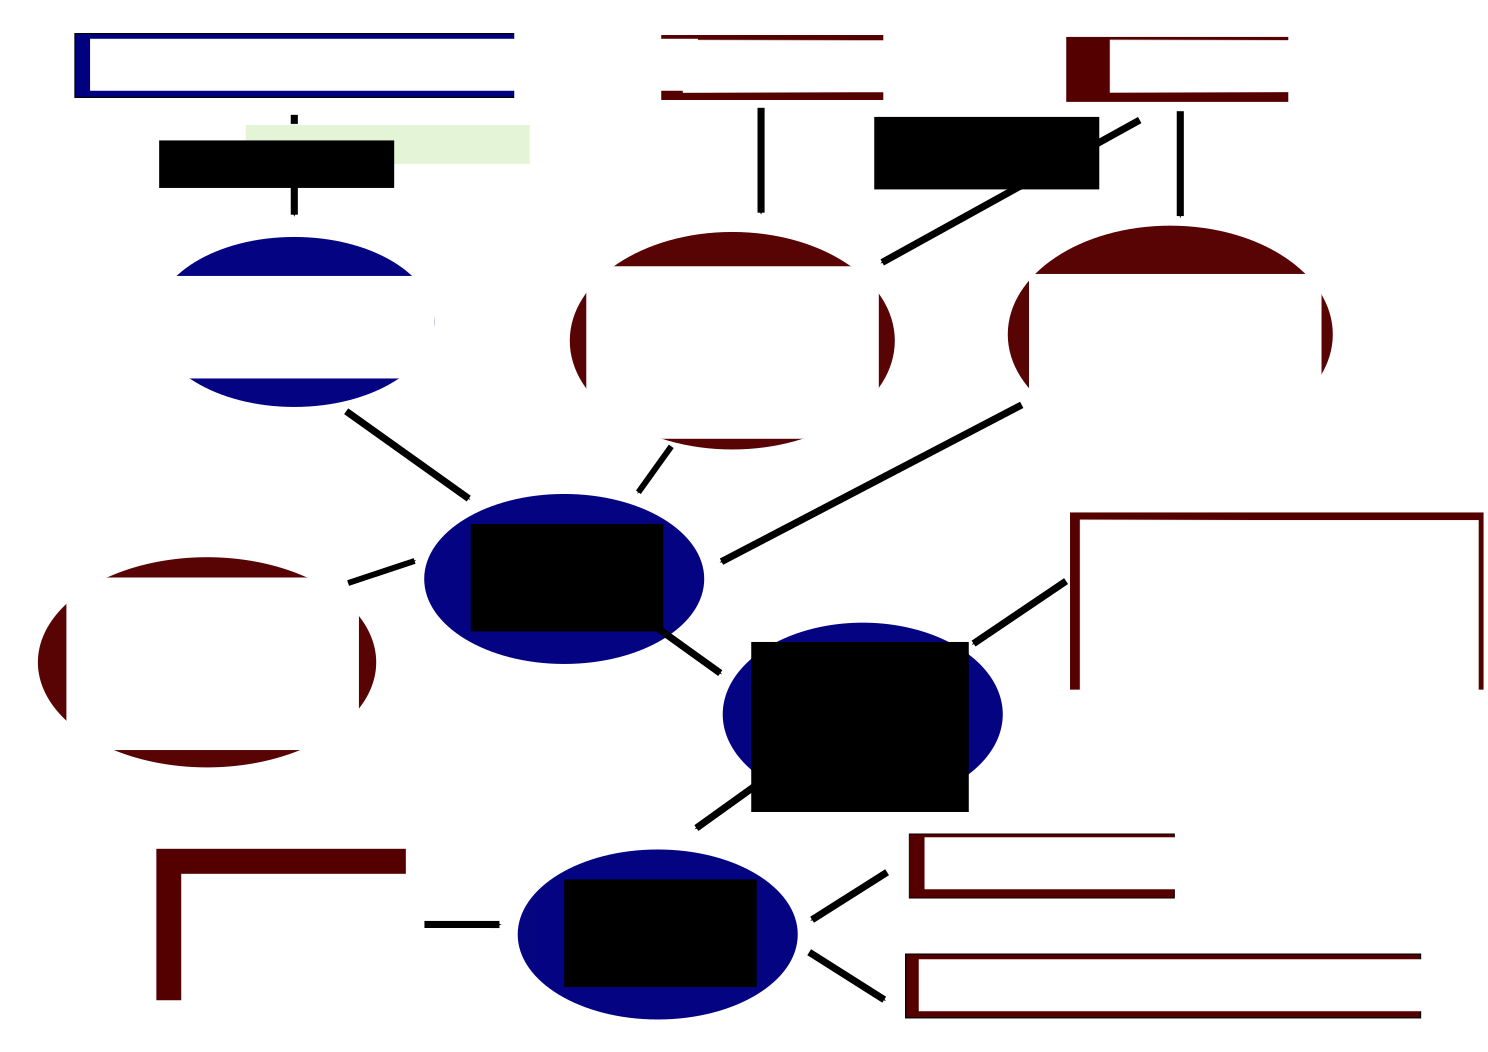
\includegraphics[scale=0.27]{moses_paraphrasing.png} 
\caption{Pipeline of Moses adjusted for the targeted monolingual translation.
Changes to the original Moses pipeline (\Fref{moses_simple}) are highlighted by
the brown colour.}
\label{moses_paraphrasing}
\end{center}
\end{figure*}

\subsubsection{Language model}
We create the language model (LM) using SRILM  \cite{srilm}, a toolkit for 
building and applying statistical language models, on the data from the Czech 
part of the Czech-English parallel corpus CzEng \cite{czeng}. 

\subsubsection{Translation models}
Each entry in Moses phrase tables contains a phrase, its translation, several
feature scores (translation probability, lexical weight etc.), and optionally
also alignment within the phrase and frequencies of phrases in the training 
data. The phrase tables are learned automatically from large parallel data.
As we do not have any large corpora of Czech-Czech parallel data, we create the 
following two ``fake'' translation tables for paraphrasing from Czech WordNet
and the Meteor paraphrase tables.

\subsubsection*{Enhanced Meteor table}
The enhanced Meteor table was created from the Czech Paraphrase Meteor tables. Each 
paraphrase pair comes with a pivoting score (see Section \ref{Data}) which we 
adapt as a feature in out phrase table. 

We also add our own paraphrase scores, acquired by \textit{distributional 
semantics}. Distributional semantics assumes that two phrases are semantically 
similar if their contextual representations are similar. \cite{miller-91}

We collect all contexts (words in a window of limited size) in which Meteor 
paraphrases occur in the Czech National Corpus \cite{SYN2010} and then measure 
context similarity cosine distance, taking into account the number of word 
occurrences) for each pair of paraphrases. 

We add six scores for each pair of paraphrases according to the size of the 
context window used (1-3 words) and whether word order played a role in the 
context. Several lines from the Enhanced Meteor table are presented in 
\Fref{moses_tables}.

\subsubsection*{One-word paraphrase table}
We create second phrase table from Czech WordNet and the filtered Meteor.
It contains only one-word pairs and thus decreases the advantage of using
a phrase translation system. However, it is designed to compensate for
the noise in the Enhanced Meteor table (see Section \ref{Data}).

We first create a set of all words from Czech side of CzEng appearing at 
least five times to exclude rare words and possible typos. We also add all 
words appearing in the MT outputs and the reference sentences. Morphological 
analysis of the words was then performed using Morče \cite{morce:2007}. 

For every word $ x $ from this set, we add to this translation table every pair 
of words that fulfils at least one of the following requirements:

\begin{itemize}
\item $ x,x $ (not every word should be paraphrased)
\item $ x,y $, if $ x $ has the same lemma as $ y $ (some word 
might have different morphology in the paraphrased sentence)
\item $ x,y $, if lemma of $ x $ and lemma of $ y $ are paraphrases according 
to Czech WordNet PDT 1.9.
\item $ x,y $, if lemma of $ x $ and lemma of $ y $ are paraphrases according 
to the filtered Meteor.
\end{itemize}

These categories constitute the first four scores in the phrase table. A pair 
of words gets score $ e $ if these words fall to a given category, 1 ($e^0$) 
otherwise.\footnote{Phrase-table scores are considered log-probabilities.} 
This phrase table contains more than a million pairs of words.

We add another score expressing POS tag similarity between the two words. It is 
computed $ e^{\frac{1}{a+1}}$, where $ a $ is the minimal Hamming distance 
between tags of the words. This probability should reflect how morphologically 
distant the paraphrases are. 

\subsubsection{Feature for targeted paraphrasing}
In order to steer the MT decoder (translation engine) in the direction of the 
hypotheses, we implemented to Moses an additional feature, which measures the 
overlap with the hypothesis. In order to keep its computation tractable during 
search, the overlap is defined simply as the number of words from the 
hypothesis confirmed by the reference translation.  Our code is included in
Moses.\footurl{https://github.com/moses-smt/mosesdecoder/blob/master/moses/FF/CoveredReferenceFeature.cpp}

%Integration into the beam search algorithm used in phrase-based decoding
%requires us to keep track of feature state (i.e. reference words covered) to
%allow for correct hypothesis recombination. We also implemented an estimator of
%future phrase score, defined as the number of reference translation words
%covered by the given phrase.

\subsubsection{Parameter tuning}

\begin{table*}[tb]
%\begin{center}
\begin{tabular}{r|l|c|c}
setting & reference sentence used & correlation & avg. BLEU \\
\hline
\textbf{Baseline} & original reference sentence, no paraphrasing & \textbf{0.75} & 12.8 \\
\textbf{Paraphrased} & paraphrased by Moses using MERT-learned weights  & 0.50  & 15.8 \\
\textbf{LM+0.2}  & paraphrased by Moses with LM weight increased by 0.2  & 0.24 & 9.1 \\
\textbf{LM+0.4} & paraphrased by Moses with LM weight increased by 0.4  & 0.22 & 6.7 \\
\end{tabular}
\caption{Description of the basic settings and the results - Pearson's 
correlation of BLEU and the human judgment, the average BLEU scores.} 
%korelace metrik - 0.981
\label{moses_settings}
%\end{center}
\end{table*}


\begin{figure*}[tb]
\begin{center}
\begin{tabular}{l|r}
 \textbf{Source } &  \textit{Paclík claims he would dare to manage the association.} \\
 \hline
 
 \textbf{Baseline} & Paclík tvrdí , že by si na vedení asociace troufl.\\
           & \textit{Paclík claims he would dare to lead the association.} \\

 \hline
 \textbf{Hypothesis} & Paclík tvrdí, že by se odvážil k řízení komory. \\
            & \textit{Paclík claims he would find the courage to control the chamber.}  \\ 

 \hline
 \textbf{Paraphrased} & Paclík tvrdí, že by se na řízení organizace troufl. \\
             & \textit{*Paclík claims he would dare to control the organization.}\\
 \hline 
 \textbf{LM+0.2} & Paclík tvrdí, že by si troufl na řízení ekonomiky. \\
               &\textit{ Paclík claims he would dare to control the economy.} \\
  
\hline 
 \textbf{LM+0.4} & Říká se, že Paclík si troufl na řídící rady. \\
               & \textit{They say that Paclík ventured to governing boards.} \\
%Lexical & Paclík tvrdí , že by se na řízení asociace troufl .\\
%Lexical boosted by 20 & Paclík tvrdí , že by si troufl na řízení ekonomiky .\\
%asociace, komora nikde nejsou jako parafraze

\end{tabular}
\caption{Example of the targeted paraphrasing using Moses. The~hypothesis is 
a correct translation of the source sentence. The new paraphrased reference 
is slightly closer in wording to the hypothesis, but there is an error due to 
a bad word choice. The sentences created with increased weights of the 
language model are both grammatically correct, but the sentence lost its 
original meaning. In the \textbf{LM+0.4} setting, they also differ a lot in 
wording from both the hypothesis and the reference sentence.}
\label{example:Moses}
\end{center}
\end{figure*}

We use the minimum error rate training (MERT) \cite{mert} to find the optimal 
weights for our models. MERT asserts the weights to maximize the translation 
quality, which is measured with BLEU. We use the reference sentences and the 
highest rated MT output from WMT12 as the parallel development data for tuning. 

This method, however, turned out not to be optimal for our setting. The feature 
for targeted paraphrasing naturally obtains the highest weight (0.51) as it 
provides an oracle guide towards the hypothesis. On the other hand, the language 
model get very small weight (0.016).

As a result, the paraphrased sentences tend to be closer to the hypothesis, but 
not grammatically correct. Therefore, we experiment with increasing the weight 
of the language model manually. 

\subsubsection{Results}
We compare four different basic settings, the results are presented in 
\Tref{moses_settings}. In contrast to our previous results, the baseline score 
is not exceeded by any of our paraphrasing methods. \Fref{example:Moses} 
represents an example of outputs. 
%A visualization of the results is shown in \Fref{visualization}. 

There are several reasons for the clear decrease in correlation with 
paraphrased references. Hypotheses generated by the \textbf{Paraphrased} 
setting, while obtaining a significantly higher BLEU score, were mostly 
ungrammatical and reduced the correlation of our metric.

The small weight of the language model seems to be the problem, but its 
increase brings even more chaos. It creates hypotheses which are nice and 
grammatically correct but often wholly unrelated to the source sentence.

This shows that our paraphrase table noise filtering was by no means sufficient 
and there is a lot of noise in our phrase tables-- given the high weight for the 
targeted paraphrase feature, we essentially transform the correct reference 
sentences to incorrect hypotheses at all cost, using our noisy phrase tables.

Our targeting feature is not ideal -- it ignores word order and operates
only on the word level (it does not model phrases). Ungrammatical translations
with scrambled word order are considered perfectly fine as long as the
translation contains the same words as the reference. So while the feature 
for targeted paraphrasing does provide a kind of oracle, it does not guarantee 
reaching the best possible translation in terms of BLEU score, let alone a 
grammatical translation.

Another problem is illustrated by very small weights assigned to our 
translation models. In fact, the highest weight among translation model 
features was assigned to the tag similarity feature (0.031). This shows 
that our model features (pivoting score, distributional similarity scores, ...) 
fail to distinguish good paraphrases from the noise. 

The combination of noise in the translation tables and the boosted language
model then causes that the most common paraphrase according to the language 
model with a similar tag gets the preference. 

\subsection{Paraphrasing via Treex}
\begin{figure*}[tb]
\begin{center}
%\scalebox{0.89}{
%\begin{tabular}{l|l}
 \begin{tabular}{l|l}
 Source &  \begin{tabular}{l}
  	\textit{The Internet has caused a boom in these speculations.} \\
	\end{tabular} \\
 \hline
 
 Hypothesis & \begin{tabular}{lllllll}
 			Internet & vyvolal & boom & v  & t\v{e}chto & spekulac\'{i}ch & . \\
 			\textit{Internet} & \textit{caused} & \textit{boom} & \textit{in} & \textit{these} & \textit{speculations} & \textit{.}\\
			\end{tabular} \\
 &  \begin{tabular}{l}
  	\textit{The Internet has caused a boom in these speculations. }\\
	\end{tabular} \\

 \hline
 %\noindent\rule{8cm}{0.4pt}\\
 Reference & \begin{tabular}{llllll}
 			Rozkv\v{e}t & t\v{e}chto & spekulac\'{i} & zp\r{u}sobil & internet & .  \\
 			\textit{Boom} & \textit{these} &  \textit{speculations} & \textit{caused} & \textit{internet} & \textit{.} \\
			\end{tabular} \\
 &  \begin{tabular}{l}
  	\textit{Boom of these speculation was caused by the Internet.} \\
	\end{tabular}  \\ 

\end{tabular}

\vspace{20pt}

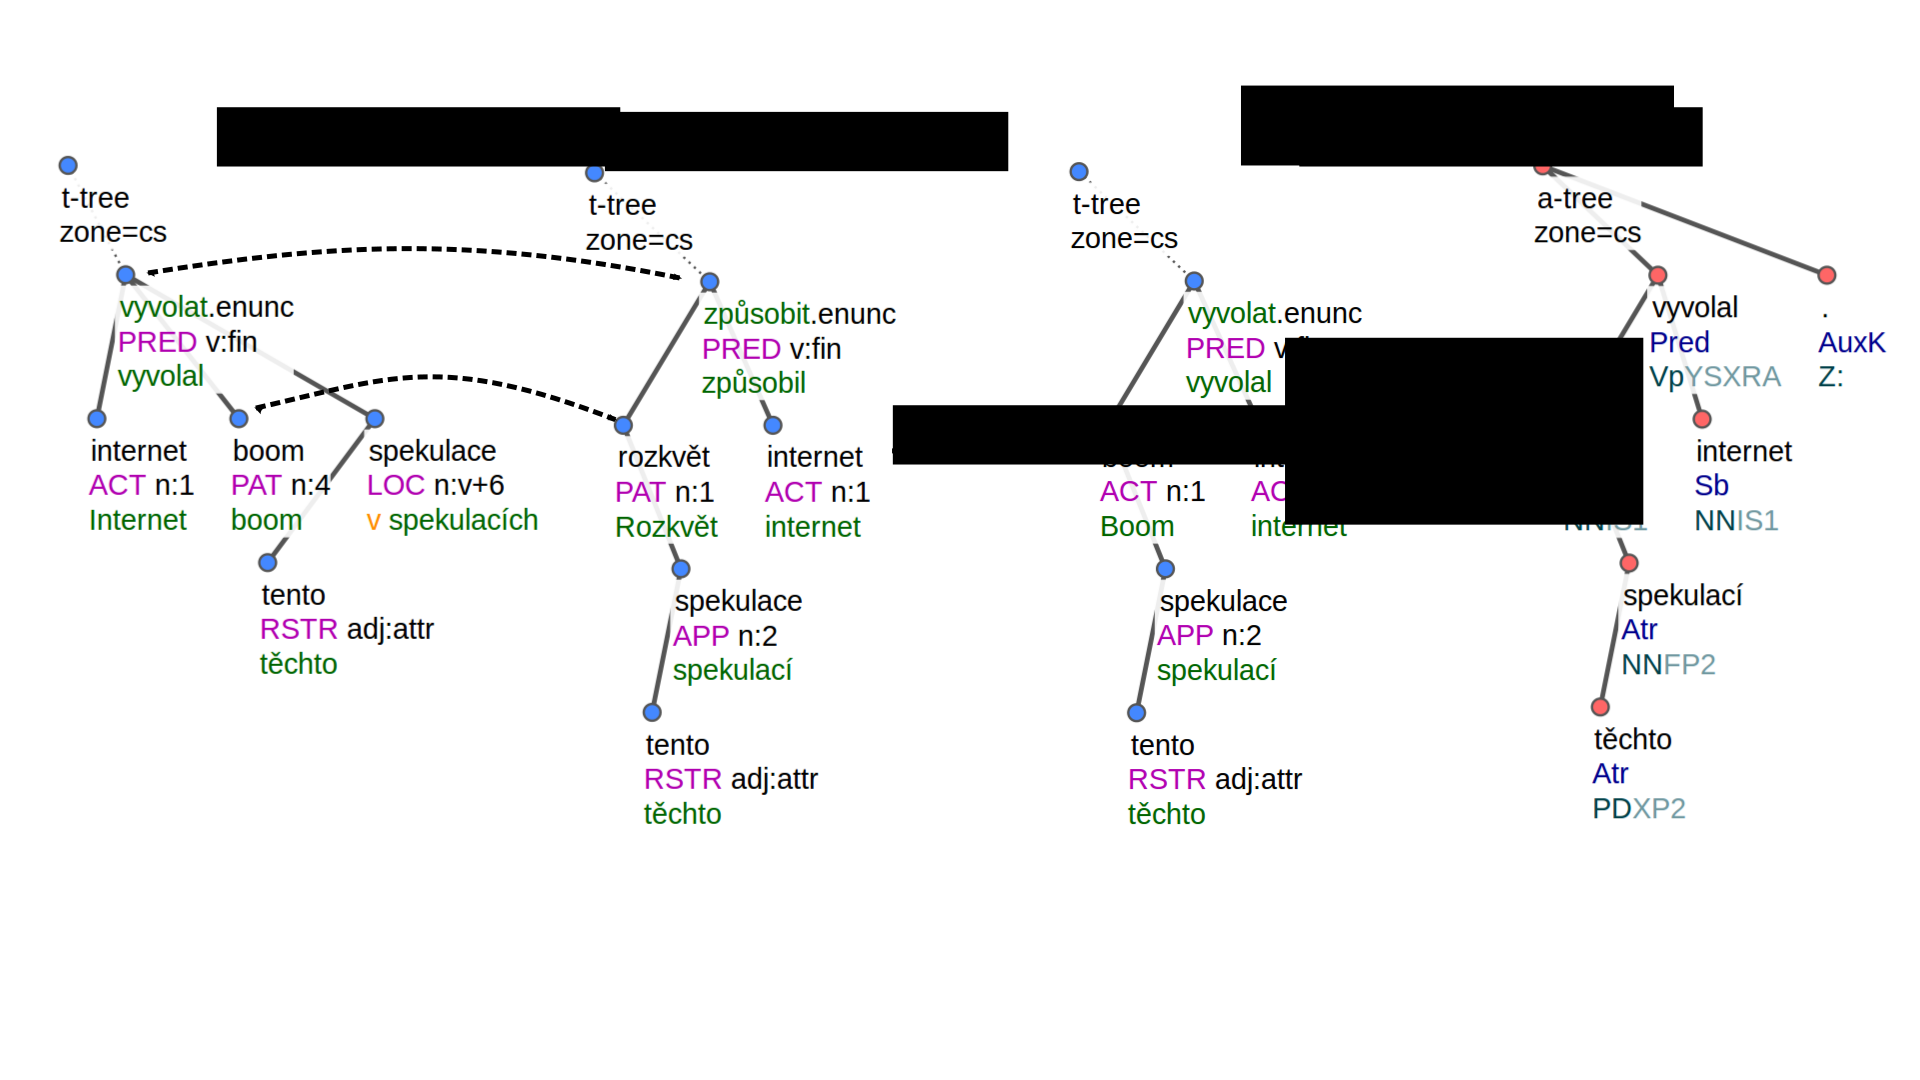
\includegraphics[scale=0.4]{example.png} 

\caption{Example of the paraphrasing. The~hypothesis is grammatically correct 
and has very similar meaning as the reference sentence.  We analyse both 
sentences to t-layer, where we create new reference sentence by substituting
synonyms from hypothesis to the reference. In the next step, we will change also
the word order to better reflect the hypothesis.}
\label{treex_example}
\end{center}
\end{figure*}

Based on the previous results, Moses does not seem to be an optimal tool for 
our task, unless we create less noisy phrase tables and a better targeting 
feature, and unless we employ another function for tuning weights. 
%TODO: lepsi tuning? e.g. MIRA 

However, there is another solution to a phrase-based translation system -- 
namely a rule-based machine translation system TectoMT \cite{tectomt}, which is 
included in a highly modular NLP software system Treex \cite{treex}.

Treex implements the stratificational approach to language, adopted from the 
Functional Generative Description theory \cite{FGP} and its later extension 
applied in the Prague Dependency Treebank \cite{PDT3.0}. It represents 
sentences at four layers: 
\begin{itemize}
\item \textbf{w-layer:} word layer; no linguistic annotation
\item \textbf{m-layer:} morphological layer; sequence of tagged and lemmatized 
words
\item \textbf{a-layer:} shallow-syntax/analytical layer; sentence is 
represented as a surface syntactic dependency tree
\item \textbf{t-layer:} deep-syntax/tectogrammatical layer; sentence is 
represented as a dependency tree, where autosemantic words only have their own 
nodes; t-nodes consist of a t-lemma and a set of attributes -- a \textit{formeme} 
(information about the original syntactic form) and a set of \textit{grammatemes} 
(essential morphological features).
\end{itemize} 

In TectoMT \cite{tectomt}, a sentence in a source language is analyses from 
the w-layer to the t-layer, where is transferred to the t-layer of a target 
language, and then generated to the w-layer of the target language. 

Our analysis and generation pipeline is taken from the TectoTM system. In our 
setting, we transfer a hypothesis and a corresponding reference sentence to 
the t-layer, where we replace the transfer phase with a module for t-lemma 
paraphrasing. After paraphrasing, we perform synthesis to a-layer, where we 
plug in a reordering module and continue with synthesis to the w-layer. 

This way, we can easily overcome some of the problems of paraphrasing using 
Moses. Most importantly, we can compare two sentences only and there is no need 
to create translation tables, thus less space for the noise to interfere. Also 
there already is highly developed machinery to avoid ungrammatical sentences. 

Treex is opensource and is available on GitHub\footurl{https://github.com/ufal/treex}, 
including our modifications.

\subsubsection{Analysis from w-layer to t-layer}
The analysis from the w-layer to the a-layer includes tokenization, POS-tagging
and lemmatization using MorphoDiTa \cite{morphodita}, dependency parsing using
the MSTParser \cite{McDonald:2005} adapted by \newcite{Novak:2007}, trained on
PDT.

A surface-syntax a-tree is then converted into a deep-syntax t-tree. Auxiliary 
words are removed, with their function now represented using t-node attributes 
(grammatemes and formemes) of autosemantic words that they belong to (e.g. two
a-nodes of the verb form \textit{spal jsem} (``I slept'') would be collapsed 
into one t-node \textit{spát} (``sleep'') with the tense grammateme set to 
past; \textit{v květnu} (``in May'') would be collapsed into \textit{květen} 
(``May'') with the formeme \textit{v+X} (``in+X'').

%tady zminit proc vlasne chceme parafrazovat pres tektokgramatickou rovinu
% jednak existuji scenare pro cestu tam a dolu a jednak na te rovine jsou slova
% zbavena uz prakticky vsech syntaktickych informaci. 
We choose the t-layer for paraphrasing, because the words from the sentence 
are lemmatized with their syntactical information hidden in formemes. 
Furthermore, functional words, which we do not want to paraphrase and that 
cause a lot of noise in our paraphrase tables, do not appear here.
%TODO: Furthermore the syntactic information of the original sentence is hidden
%inside the grammatemes. And really do not want to change them (mozna nejaky
%ty diathese, to se uvidi)
\begin{figure*}[tb]
\begin{center}
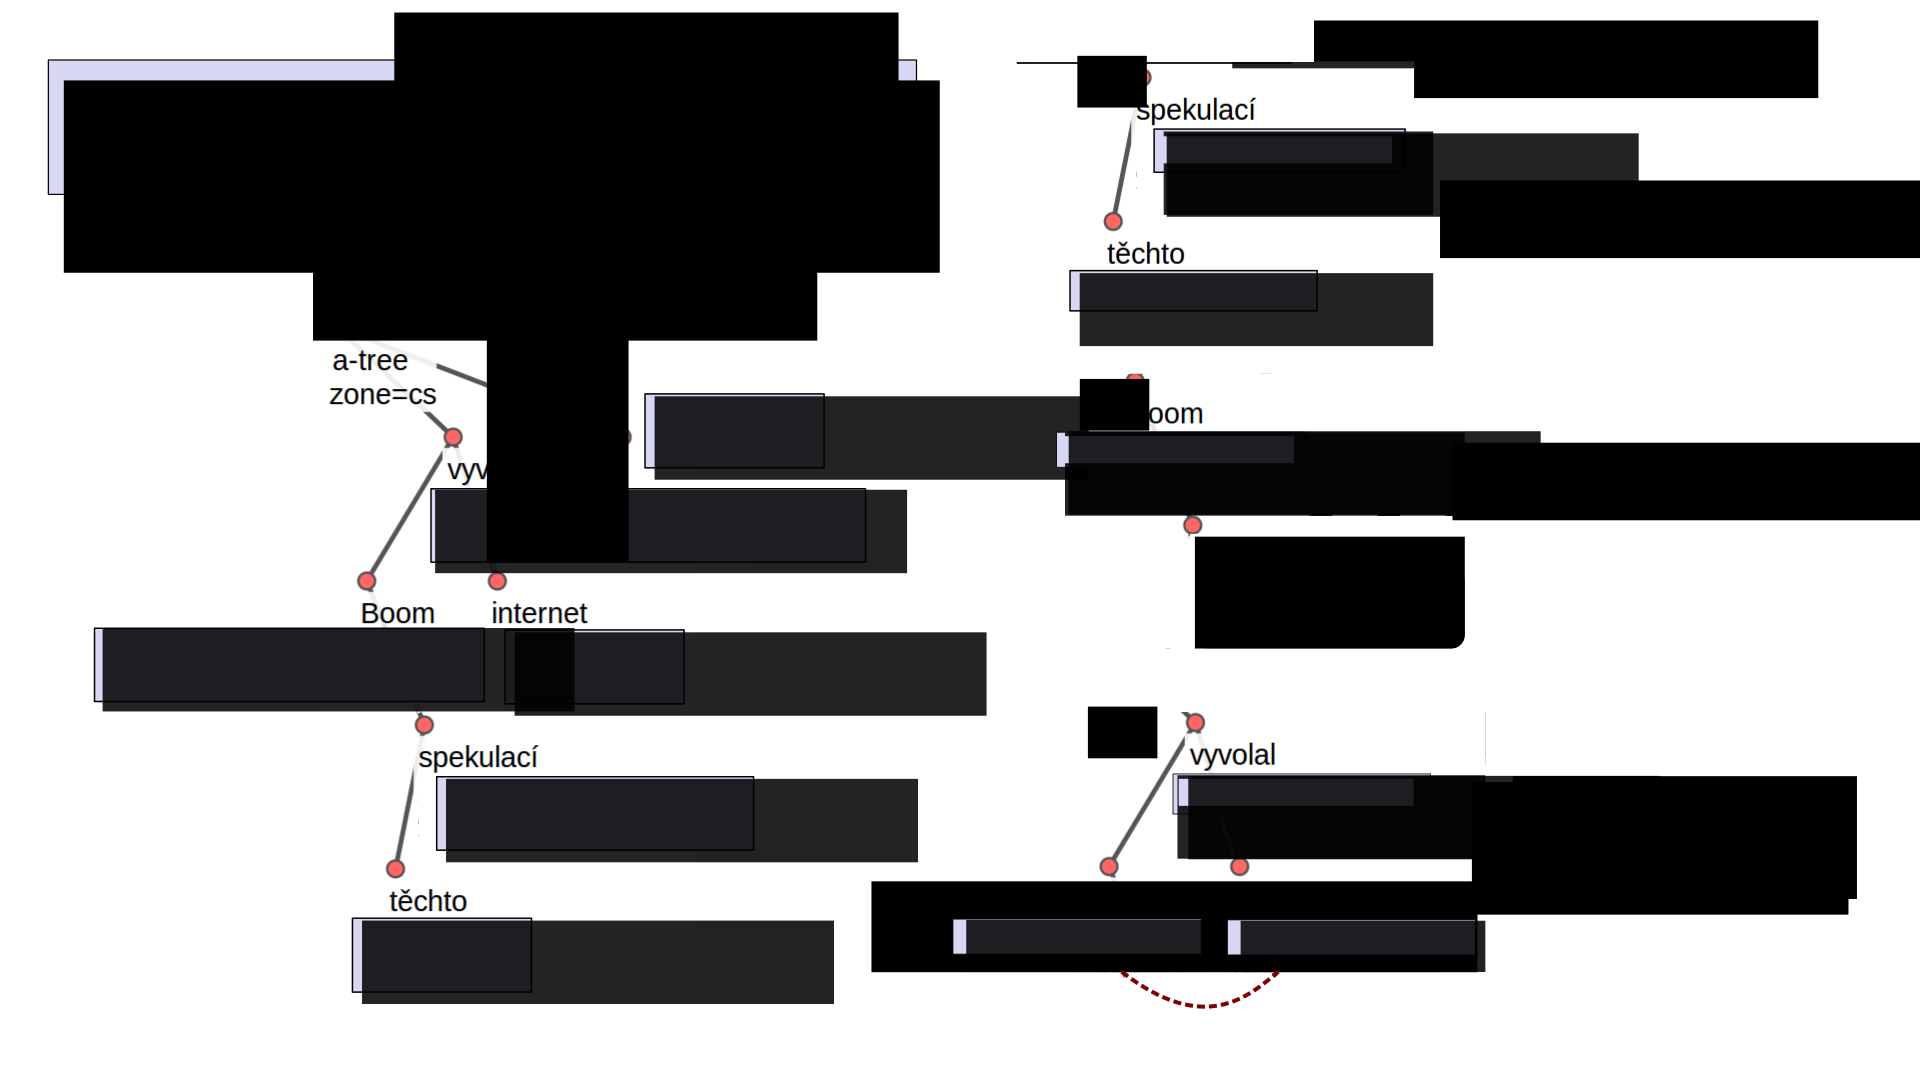
\includegraphics[scale=0.32]{reordering.png} 
\caption{Continuation of \Fref{example:Moses}, reordering of the paraphrased reference
sentence.}
\label{reordering}
\end{center}
\end{figure*}

\subsubsection{Paraphrasing}
The paraphrasing module T2T::ParaphraseSimple is freely available at 
GitHub.\footurl{https://github.com/ufal/treex/blob/master/lib/Treex/Block/T2T/ParaphraseSimple.pm} 

T-lemma of a reference t-node is changed from A to B if and only if:
\begin{enumerate}
\item there is no hypothesis t-node with lemma A
\item there is a hypothesis t-node with lemma B 
\item there is no reference t-node with lemma B
\item A and B are paraphrases according to our paraphrase tables
\end{enumerate}

The other attributes of the t-node are kept unchanged based on the theory that
semantic properties are independent of the t-lemma. However, in practice, this 
is not always true: t-nodes corresponding to nouns are marked for grammatical 
gender, which is very often a grammatical property of the given lemma with no 
effect on the meaning (for example, ``a house'' can be translated either as a 
masculine noun \textit{dům} or as feminine noun \textit{budova}).
%; we really believe this should be marked on the lemma only, but this is not the case in Treex. 

Therefore, when paraphrasing a t-node that corresponds to a noun, we delete 
the value of the gender grammateme, and let the subsequent synthesis pipeline 
generate the correct value of the morphological gender feature value (which is 
necessary to ensure correct morphological agreement with surrounding words, 
such as adjectives and verbs).

\subsubsection{Synthesis from t-layer to a-layer}
In this phase, a-nodes corresponding to auxiliary words and punctuation are 
generated, morphological feature values on a-nodes are initialized and set to 
enforce a morphological agreement among the nodes. Correct word forms based 
on lemmas and POS, and morphological features are generated using MorphoDiTa.

\subsubsection{Tree-based reordering}
The reordering block A2A::ReorderByLemmas is freely available at 
GitHub.\footurl{https://github.com/ufal/treex/blob/master/lib/Treex/Block/A2A/ReorderByLemmas.pm}

The idea behind the block is to make the word order of a new reference as 
similar to the word order of the translation as possible, but with some 
tree-based constraints to avoid ungrammatical sentences. 

The general approach is to reorder the subtrees rooted at modifier nodes of a 
given head node so that they follow in an order that is on average similar to 
their order in the translation. \Fref{reordering} shows the reordering process 
of the a-tree from \Fref{treex_example}.

%As the ultimate MT quality metric we apply to compare the translation and
%he reference is word based, we align translation and reference words that have
%an identical lemma. Reordering reference words with a lemma that does not
%appear in the translation has little effect on the resulting score given by the
%metric, we thus treat those as unaligned words. %For simplicity, we also treat
%repeated words as unaligned, as it is not straightforward to decide which of 
%the possible alignments to use; however, repeated words are rather rare. 
%TODO future work – align more words.

Our reordering proceeds in several steps. Each a-node has an order, i.e. its 
position in the sentence.  We define the \emph{MT order} of a reference 
a-node as the order of its corresponding hypothesis a-node, i.e. node a node 
with the same lemma. 

We set the MT order only if there is exactly one a-node with the given lemma 
in both the hypothesis and the reference. Therefore, the MT order might be 
undefined for some nodes.

In the next step, we compute the \emph{subtree MT order} of each reference 
a-node R as the average MT order of all a-nodes in the subtree rooted at the 
a-node R (including the MT order of R itself). Only nodes with a defined MT 
order are taken into account, so the subtree MT order can be undefined for 
some nodes. 

Finally, we iterate over all a-nodes recursively starting from the bottom. Head 
a-node $H$ and its dependent a-nodes $D_i$ is reorder if they violate the
\emph{sorting order}. If $D_i$ is a root of a subtree, the whole subtree is 
moved and its internal ordering is kept.

The sorting order of $H$ is defined as its MT order; the sorting order of each 
dependent node $D_i$ is defined as its subtree MT order. If a sorting order of 
a node is undefined, it is set to the sorting order of the node that precedes 
it, thus favouring neighbouring nodes (or subtrees) to be reordered together in 
case there is no evidence that they should be brought apart from each other. 
Additionally, each sorting order is added 1/1000th of the original order of the 
node -- in case of a tie, the original ordering of the nodes is preferred to 
reordering.

We do not handle non-projective edges in any special way, so they always get 
projectivized if they take part in a reordering process, or kept if they do
not. However, no new non-projective edges are created in the process – this is
ensured by always moving the subtrees at once.

Please note that each node can take part in at most two reorderings – once
as the $H$ node and once as a $D_i$ node. Moreover, the nodes can be processed 
in any order, as a reordering does not influence any other reordering.

\subsubsection{Synthesis from a-layer to w-layer}
The word forms are already generated on the a-layer, so there is little to be 
done. Superfluous tokens are deleted (e.g. duplicated commas), prepositions are
vocalized, the sentence beginning is capitalized, and the tokens are 
concatenated (a set of rules is used to decide which tokens should be
space-delimited and which should not).

The example sentence (from \Fref{reordering}) results in the following sentence:
\textit{Internet vyvolal boom těchto spekulací} (``The Internet has caused a boom 
of these speculations.''), which has the same meaning as the original reference 
sentence, is grammatically correst and most importantly is much more similar in
wording to the hypothesis.

%ref: Rozkvět těchto spekulací způsobil internet.
%mt: Internet vyvolal boom v těchto spekulacích.
%before reordering těchto spekulací vyvolal internet.
%final: Internet vyvolal boom těchto spekulací.

\subsubsection{Results}
\begin{table*}[tb]
\begin{center}


\begin{tabular}{|c|ccc|ccc|}
\hline
\multicolumn{1}{|l|}{} & \multicolumn{3}{c|}{\textbf{WMT12}}   & \multicolumn{3}{c|}{\textbf{WMT13}}  \\ 
\hline
references             & original & paraphrased & reordered & original & paraphrased & reordered \\ 
\hline
BLEU                   & 0.751    & 0.783       & 0.804     & 0.834    & 0.850       & 0.878   \\  %0.852  
Meteor                 & 0.833    & 0.864       & 0.870     & 0.817    & 0.871       & 0.870   \\  %O.871
Ex.Meteor              & 0.861    & 0.900  & \textbf{0.904} & 0.848  & \textbf{0.893} & \textbf{0.893}\\  %0.891
\hline
\end{tabular}
\caption{Pearson correlation of a metric and human judgment on original 
references, paraphrased references and paraphrased reordered references. 
Ex.Meteor represents Meteor metric with exact match only (i.e. no paraphrase
support).}
\label{results:treex}
\end{center}
\end{table*}

We evaluate the new paraphrased references with three different metrics -- BLEU, 
Meteor and the Meteor metric without the paraphrase support (based on \Sref{parmesan} 
and the fact that it seem redundant to use paraphrases on already paraphrased 
sentences). 
%TODO asi by to chtelo zaradit vic metrik, kdyz se tim tak chlubim
% idealne nejakou tu "hlubokou", napr. semPOS

The results are presented in \Tref{results:treex} as a Pearson correlation of a 
metric with human judgment. Contrary to Moses results (\Tref{moses_settings}), 
paraphrasing using Treex clearly helps to reflect the human perception better. 

However, the results are worse than the Simple substitution method (\Sref{lrec}),
even though they essentially perform similar task -- one-word substitution. One 
reason of the different performance is smaller number of substitutions, only 
1.39 (WMT12)/ 1.12 (WMT13) word per sentence.

We find some problem with punctuation (e.g., the exclamation marks are missing)
and 
One reason of the different performance is smaller number of substitutions, 
only 1.39(WMT12)/ 1.12(WMT13) word per sentence.

%Model as described hardly employs all possibilities of Treex - we
% still do only one to one substitution. We plan to extend it....BLAH

The reordering clearly helps when we evaluate via the BLEU metric, which 
punishes any word order changes to the reference sentence. Meteor is more
tolerant to word order changes and the reordering has practically no effect 
on his scores.

However, manual examination showed that our constraints are not strong enough 
to prevent creating non grammatical sentences. The algorithm tend to copy the
word order of the hypothesis, even if it is not correct. Most errors were caused
by changes of a word order of punctuation. 

TODO: There is also problems with some not commonly used phrases in the languages the synthesis
can not deal with very well.

%Jen si vzpomeňte, kolikrát jste už tomu svému řekla, ať na vás raději počká před vchodem...
%Jen nezapomenu, jak jste mnoho časů říkali své druhé polovině, čekají na vás...
%Jen vzpomeňte, kolikrát jste už tomu říkaly svých, ať čeká před vchodem na vás rád.
%Jen si vzpomeňte , kolikrát jste už tomu svému říkali , ať na vás raději čekají před vchodem ...


%16:17 sol2 paraphrasing$cat wmt12.prumer | prumer
%4180.08
%16:17 sol2 paraphrasing$cat wmt13.prumer | prumer
%3548.67
%16:18 sol2 paraphrasing$cat wmt14.prumer | prumer
%3787.2


\section{Future Work}
Our treex model as described hardly employs all possibilities of Treex - we
only do simple one-word substitutions. In our future work, we plan to extend 
the paraphrasing pipeline for more complex paraphrases including syntactical 
paraphrases, multiword phrases, light verbs construction, diatheses, deleting 
unnecessary words, etc.

We plan to revise the word ordering scheme and add rule-based constrains to 
stop ungrammatical constructions. Furthermore, we would like to learn 
automatically possible word order changes from Deprefset \cite{bojar-scratching}, 
which contains an excessive number of manually created reference translations 
for 50 Czech sentences.

We can change only parts of sentences that are dependent on 
paraphrased words, thus keeping the rest of the sentence correct and 
creating more conservative reference sentences and avoiding bringing
mistakes during synthesis.

We perform our experiment using Treex on Czech language, but the procedure is 
generally language independent, as long as there is analysis and synthesis 
support for particular language in Treex. Currently there is full support for 
Czech, English, Portuguese and Dutch, but there is ongoing work on many more 
languages within the QTLeap\footurl{http://qtleap.eu/} project.

One of our problems is the noise in the paraphrase tables. We plan an automatic
filtering and including recently released paraphrase database PPDB \cite{ppdb}.
We plan an experiment of paraphrasing without paraphrase tables based on
\verb!word2vec! \cite{word2vec} similarity; or \verb!word2vec! improved by 
paraphrase tables \cite{Faruqui:Retrofitting}.

\bibliographystyle{acl}
\bibliography{biblio}
\end{document}
